\section{Method}
% \subsection{Problem Definition}
% \newcommand{\I}{\mathcal{I}}
% \newcommand{\Vobs}{\mathcal{V}_{\mathrm{obs}}}
% \newcommand{\Vaux}{\mathcal{V}_{\mathrm{aux}}}
% Given a static scene with sparse multi-view images $\I = \{ I_i \in \mathbb{R}^{H \times W \times 3} \}_{i=1}^{N}$, our goal is to predict 3D Gaussian Splatting (3DGS) representation in a fixed small number $K$ of refinement steps (iterative feed-forward), achieving high quality and fidelity without per-scene long optimization loops. This process can be represent as follows:
% \begin{equation}
%     G = 
%     \begin{cases}
%     init(\{ I_i \in \mathbb{R}^{H \times W \times 3} \}_{i=1}^{N}), & \text{initialization},\\
%     G_(i) + IR(G_i, f_i, (E_{i,nov},E_{i,rec}), & \text{otherwise}.
%     \end{cases}
% \end{equation}

% We represent the scene by a set of anisotropic Gaussians $G = \{ g_m = (\mu_m, s_m, o_m, c_m) \}_{m=1}^{M}$ with location of centers, scale, opacities, and colors; a rasterization-based differentiable renderer $R$ produces images from denoted view. A feed-forward network provide geometric prior outputs an initial 3D Gaussians, then a lightweight IR head performs $N$ small residual updates. A pre-trained Diffusion model from a pretrained model [Difix3D+] provides a generative prior used as an enhancement in under-constrained views.




\subsection{Problem Definition and Framework Overview}
\label{sec:problem_definition}

\paragraph{Problem definition} 
Given a set of uncalibrated multi-view image observations
$\mathcal{V}=\{(I_m)\}_{m=1}^{\mathcal{M}}$,
we represent a scene with 3D Gaussian Splatting (3DGS)
$\mathcal{G}=\{g_i\}_{i=1}^{N}$, where each Gaussian
$g_i=(\mathbf{x}_i,\mathbf{s}_i,\mathbf{r}_i,\mathbf{c}_i,\alpha_i)$
contains position, scale, orientation, color, and opacity. Our goal is to recover $\mathcal{G}$ that is photometrically consistent with $\mathcal{V}$,
while enabling fast inference and robustness under domain shift. A differentiable rasterizer $\mathcal{R}$ produces a rendering
$R_m=\mathcal{R}(\mathcal{G};\Pi_m)$ for camera $\Pi_m$.

%下面只修改了第一句
\paragraph{Framework overview} 
To combine feed-forward efficiency with scene-specific refinement and efficient use of generative prior, our framework consists of three components (in ~\cref{fig:overview}): 
We remove voxelization module in \cite{jiang2025anysplat} and fine-tune it as initializer $F_\phi$ of our framework, which first predicts camera poses and an initial 3DGS $\mathcal{G}^{(0)}$ from $\mathcal{V}$. On top of this, an iterative residual Gaussian head $U_\theta$ applies $T$ forward-only updates to refine the 3D Gaussians (in ~\cref{sec:iter_gaussian_head}). Meanwhile, a generative prior fusion mechanism converts diffusion-enhanced renderings into Gaussian-level cues that guide these updates (in ~\cref{sec:prior_fusion}).
This decomposition allows us to retain the speed of feed-forward inference while still with scene-adaptive refinement.
%上面加了一句

% see Appendix
% \algrenewcommand\algorithmicrequire{\textbf{Input:}}
% \algrenewcommand\algorithmicensure{\textbf{Output:}}
% % 让注释靠右显示（可选）
% %\algrenewcommand\algorithmiccomment[1]{\hfill\(\triangleright\) #1}
% % ==== body ====
% %\linenumbers
% \algrenewcommand\alglinenumber[1]{\scriptsize #1:}  % 正确

% \begin{algorithm}[t]
% \caption{GIFSplat Inference (forward-only refinement)}
% \label{alg:gif3d}
% \begin{algorithmic}[1]
% \Require Multi-view observations $\mathcal{V}=\{(I_m\}_{m=1}^M$; iterations $T$; view budget $K$; initializer $F_\phi$; update head $U_\theta$; rasterizer $\mathcal{R}$; feature extractor $\psi$; diffusion enhancer $\mathcal{E}_\phi$
% \Ensure Refined 3DGS $\mathcal{G}^{(T)}$ in step $T$
% \State $\mathcal{G}^{(0)} \gets F_\phi(\mathcal{V})$ \Comment{Initialization}
% \For{$t=0$ to $T-1$}
%   \State $\mathcal{P}^{(t)} \gets \textsc{SelectViews}(\mathcal{G}^{(t)}, \{\Pi_m\}, K)$ 
%   \For{each $m \in \mathcal{P}^{(t)}$}
%     \State $R_m^{(t)} \gets \mathcal{R}(\mathcal{G}^{(t)};\Pi_m)$
%     \State $O_m^{(t)} \gets \psi(I_m) - \psi(R_m^{(t)})$ \Comment{observation evidence}
%     \State $\tilde{R}_m^{(t)} \gets \mathcal{E}_\phi(R_m^{(t)})$
%     \State $P_m^{(t)} \gets \psi(\tilde{R}_m^{(t)}) - \psi(R_m^{(t)})$ \Comment{prior cue}
%   \EndFor
%   \For{each Gaussian $i$}
%     \State $\mathbf{o}_i^{(t)} \gets \textsc{Pool}(\{O_m^{(t)}\}_{m\in\mathcal{S}^{(t)}}, \{w_i(u)\})$ \Comment{soft assignment by rasterization weights}
%     \State $\mathbf{p}_i^{(t)} \gets \textsc{Pool}(\{P_m^{(t)}\}_{m\in\mathcal{S}^{(t)}}, \{w_i(u)\})$
%     \State $\mathcal{G}_i^{(t)} \gets U_\theta\!\big([\mathcal{G}_i^{(t)} \,\|\, \mathbf{o}_i^{(t)} \,\|\, \mathbf{p}_i^{(t)}]\big)$
%     \State $\mathcal{G}_i^{(t+1)} \gets \mathcal{G}_i^{(t)} + \mathcal{G}_i^{(t)}$ 
%   \EndFor
% \EndFor
% \State \Return $\mathcal{G}^{(T)}$
% \end{algorithmic}
% \end{algorithm}




\subsection{Iterative Gaussian Head}
\label{sec:iter_gaussian_head}

% Existing optimization-based method need long-time gradient descent to update 3D Gaussians while one-shot feed-forward method predict limited accurate results. Our goal is to achieve trade-off between performance and efficiency simultaneously. Under \emph{no} test-time backprop, this module turns the initial 3DGS $\mathcal{G}^{(0)}$ into $\mathcal{G}^{(T)}$ via $T$ forward residual updates by predicting per-Gaussian parameter increments $\mathcal{G}_i$ and enabling geometry-aware interactions within 3D neighborhoods, thereby reducing the feature discrepancy between renderings and observations; it can optionally fuse prior signals to improve robustness under domain shift. Equivalently, it forward-approximates minimizing
% $\sum_m\|\psi(I_m)-\psi(\mathcal{R}(\mathcal{G};\Pi_m))\|$,
% where $\psi$ denotes a feature extractor and $\mathcal{R}$ a differentiable renderer.
Instead of one-shot prediction, we adopt an iterative feed-forward refinement:
starting from an initialization $\mathcal{G}^{(0)}$, we apply $T$ forward update steps to obtain
$\mathcal{G}^{(T)}$, without test-time gradient backpropagation or long per-scene optimization. In short, existing paradigms satisfy only partial property at a time:
feed-forward efficiency, refinement ability, and prior utilization. We seek a formulation satisfying all three. ~\cref{fig:IR} illustrates the process of iterative refinement.

% \begin{figure}[t]
%   \centering
%   % 在双栏模板中，单栏宽度用 \columnwidth
%   \includegraphics[width=0.85\columnwidth]{pics/PAG.png}
%   \caption{Comparison of 3D Gaussian representations and interaction patterns. (a) Pixel-aligned vs. point-based Gaussians: pixel-aligned splats are tied to image grids and integrate easily with standard neural backbones, but tend to be redundant and poorly capture true 3D neighborhoods. (b) Interactions among pixel-aligned Gaussians are dense and computationally costly due to raster coupling. (c) Interactions among point-based 3D Gaussians operate in 3D space via local neighborhoods, enabling sparse, geometry-aware message passing.}
%   \label{fig:single}
% \end{figure}

\begin{figure}[t]
  \centering
  % 在双栏模板中，单栏宽度用 \columnwidth
  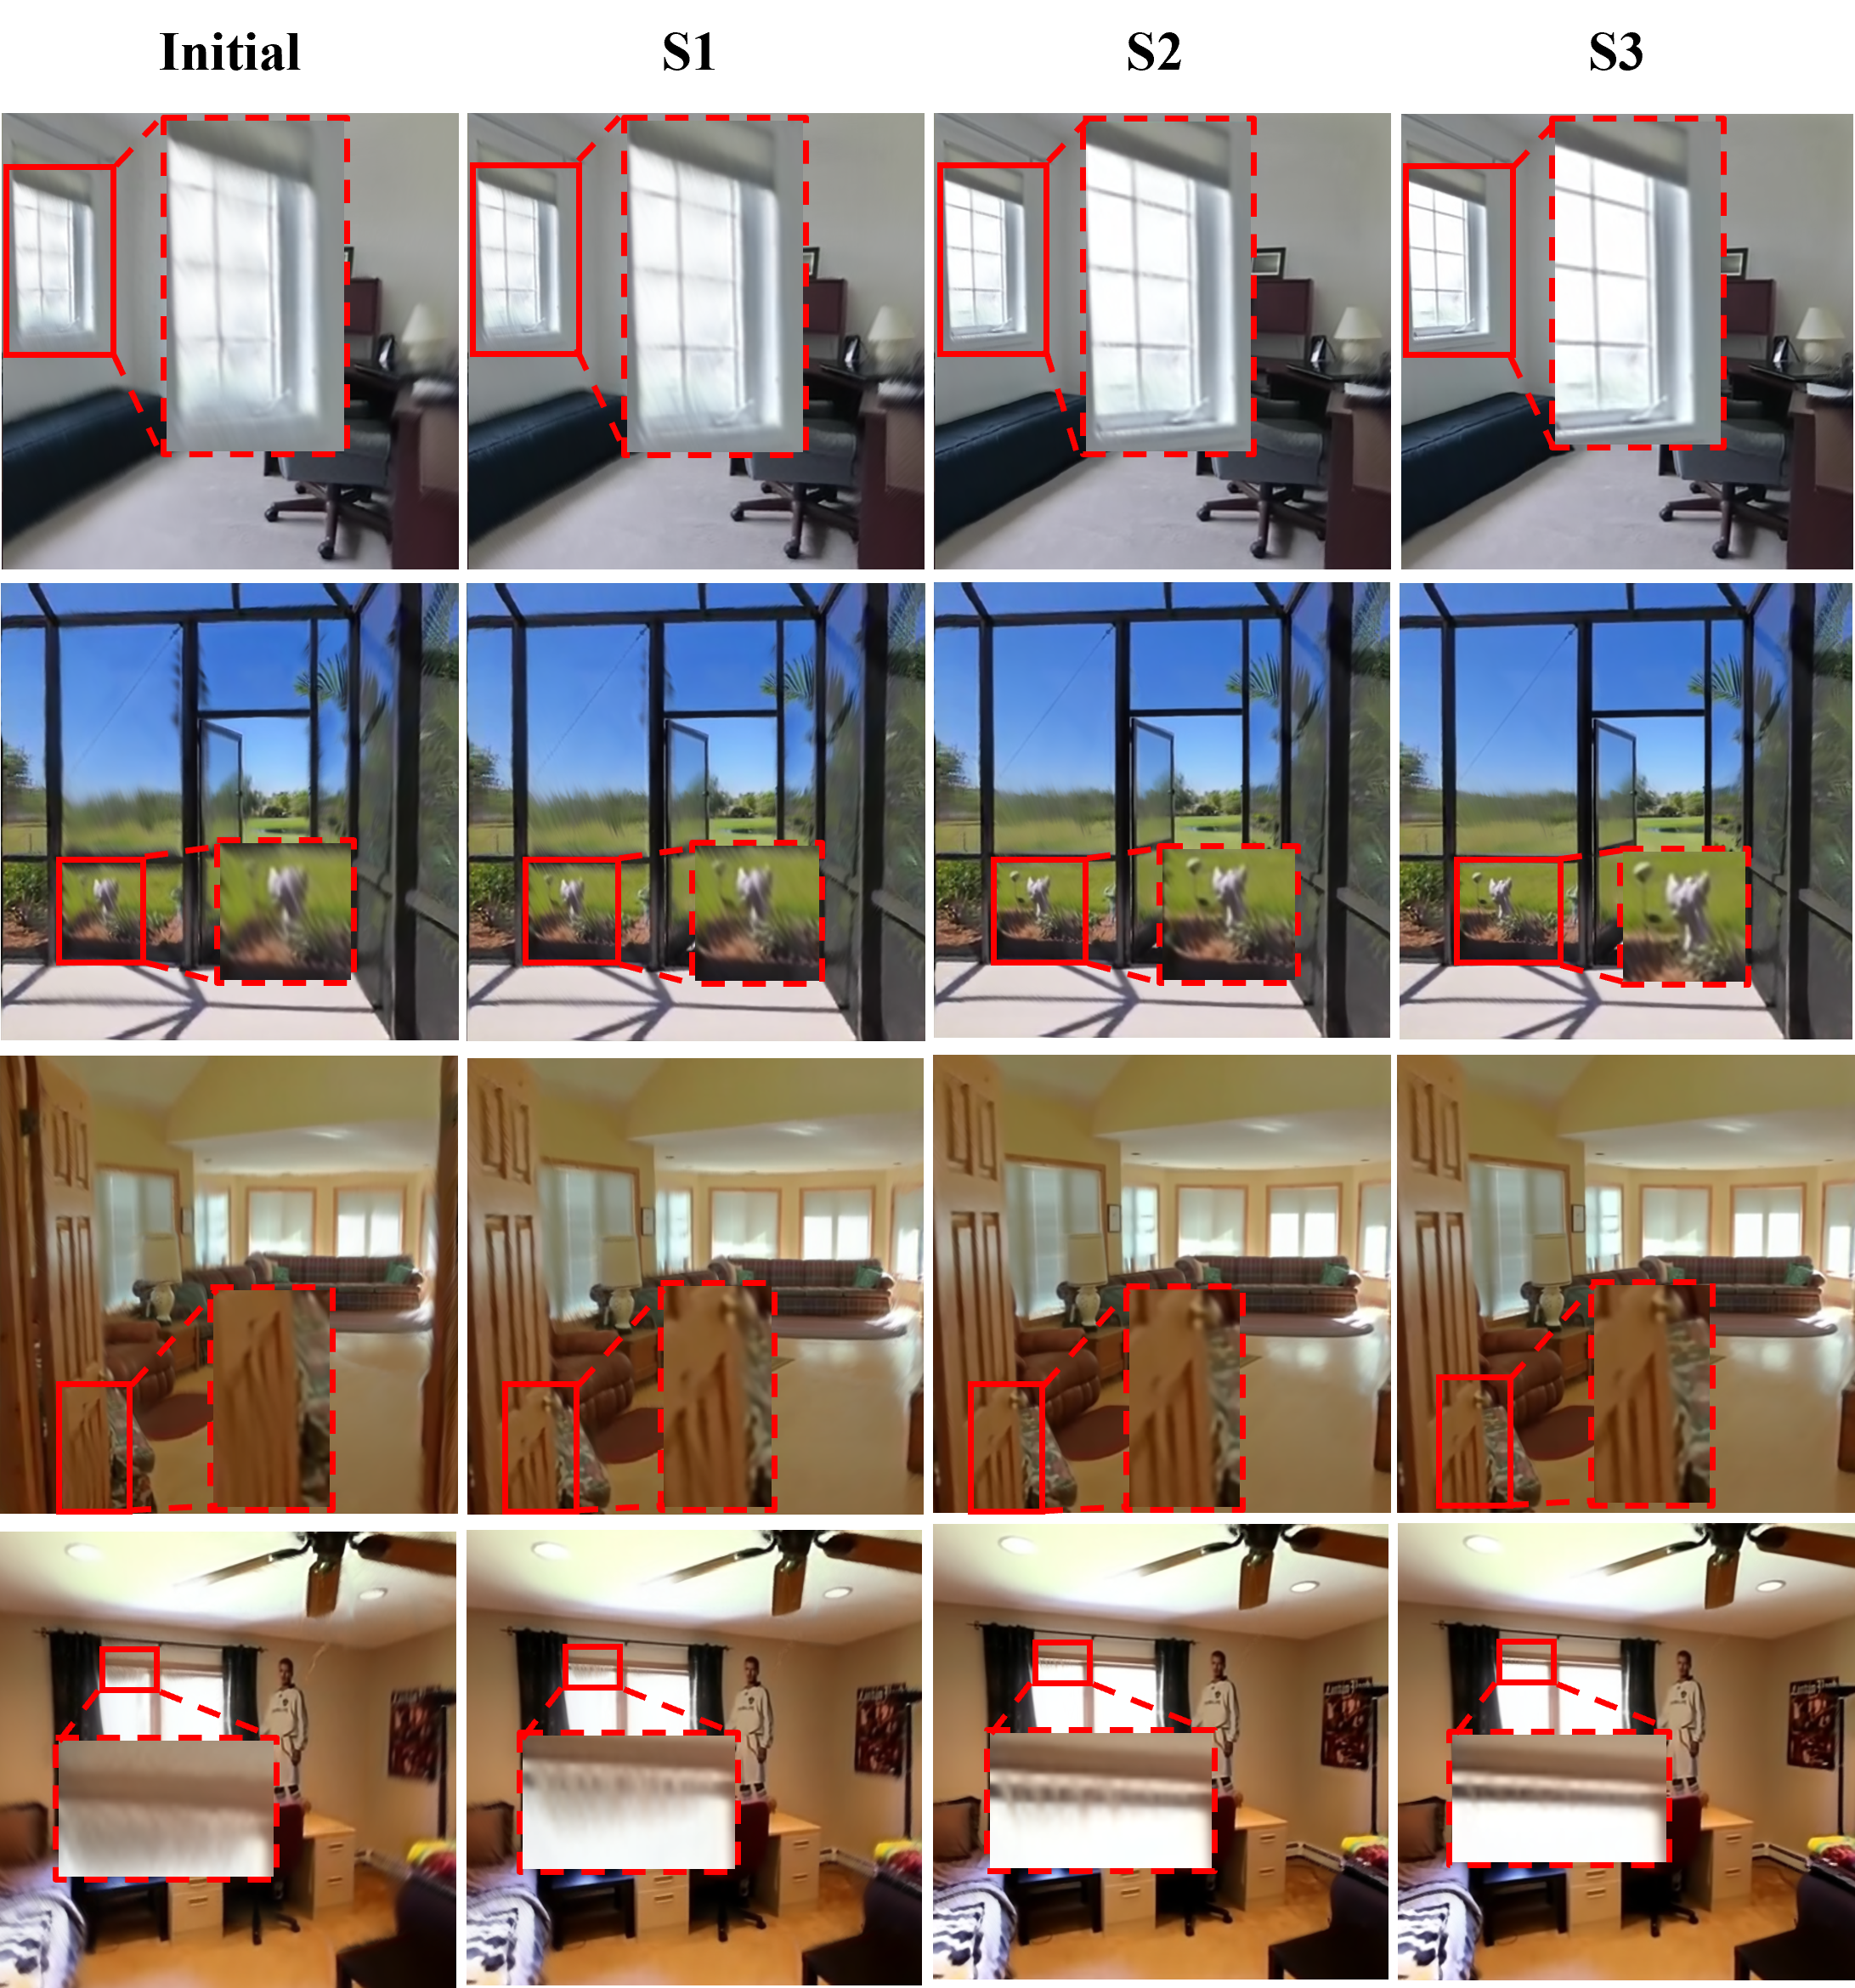
\includegraphics[width=\columnwidth]{pics/IR.png}
  \caption{\textbf{Visualizing iterative residual refinement.} Starting from the initial 3DGS prediction (left column), our iterative Gaussian head progressively refines geometry and appearance over three forward-only steps (S1–S3). The zoomed regions highlighted by red dashed boxes show reduced blur, sharper edges, and fewer artifacts as the iteration proceeds, illustrating how the proposed updates gradually improve the scene representation without test-time gradient backpropagation.}
  \label{fig:IR}
\end{figure}

Given the formulation above, we now detail how the iterative gaussian head enables
feed-forward scene refinement without test-time gradient backpropagation.
Existing optimization-based methods refine 3D Gaussians through long-time gradient
descent, whereas one-shot feed-forward models lack the ability to absorb new
evidence. Our goal is to combine their strengths: efficient inference while still allowing scene-adaptive refinement.
Under \emph{no} test-time gradients, the iterative head transforms the initial
3DGS $\mathcal{G}^{(0)}$ into $\mathcal{G}^{(T)}$ by predicting per-Gaussian residual $\{g_i\}^{(T)}$ across $T$ forward passes, reducing rendering–observation discrepancies and optionally incorporating prior cues. Equivalently, it forward-approximates minimizing
$\|\psi(I_m)-\psi(\mathcal{R}(\mathcal{G};\Pi_m))\|$, where $\psi$ is a
frozen image feature extractor and $\mathcal{R}$ is a differentiable renderer, more details are stated in Appendix.

At step $t$, the rendered views are processed by $\psi(\cdot)$ to compute feature differences $\mathcal{O}_m^{(t)}=\psi(I_m)-\psi(R_m^{(t)})$. Pixel cues are pooled to Gaussians via soft assignment weights $w_i(u)$, producing $\mathbf{o}_i^{(t)}$. 
\begin{equation}
\mathbf{o}_i^{(t)} \leftarrow
\frac{\sum_{m\in\mathcal{S}^{(t)}}\sum_{u} w_i(u)\,O_m^{(t)}(u)}
     {\sum_{m\in\mathcal{S}^{(t)}}\sum_{u} w_i(u)+\varepsilon}.
\end{equation}

The iterative gaussian head predicts residuals
$\Delta \mathcal{G}^{(t)} = \Delta \{g_i^{(t)}\}_{i=1}^{N}=(\Delta\mathbf{x}_i^{(t)},\Delta\mathbf{s}_i^{(t)},
\Delta\mathbf{c}_i^{(t)},\Delta\alpha_i^{(t)})$ and update the current 3DGS as
% \begin{equation}
%     \Delta g_i^{(t)}=(\Delta\mathbf{x}_i^{(t)},\Delta\mathbf{s}_i^{(t)},
% \Delta\mathbf{c}_i^{(t)},\Delta\alpha_i^{(t)}),
% \end{equation}
\begin{equation}
    \Delta \mathcal{G}^{(t+1)} \leftarrow U_\theta\big(\,[\mathcal{G}^{(t)} \,\|\, \{o_i\}^{(t)}]\,\big),
\end{equation}
\begin{equation}
    \mathcal{G}^{(t+1)} \leftarrow \mathcal{G}^{(t)}+\Delta \mathcal{G}^{(t)},\quad t=0,\dots,T-1.
\end{equation}

This design preserves feed-forward efficiency while providing a lightweight refinement signal on top of the one-shot initialization.

% Specifically, starting from uncalibrated sparse multi-view observations, our pipeline first produces an initial 3D Gaussian scene $\mathcal{G}^{(0)}$ from multi-view image $\mathcal{V}$ via a feed-forward initializer $F_\phi$. We then perform a short sequence of forward-only refinements. At each iteration, the current scene $\mathcal{G}^{(t)}$ is rendered from a small set of cameras $\mathcal{P}^{(t)}$ to obtain $R_m^{(t)}$, and observation-driven evidence is computed as feature differences between $R_m^{(t)}$ and the corresponding views. These pixelwise cues are softly assigned to individual Gaussians using rasterization weights. In parallel, we pass the novel view renderings through a frozen diffusion-based enhancer to obtain $\tilde{R}_m^{(t)}$; their feature-space differences provide prior cues that are pooled to Gaussians in the same way. The update head $U_\theta$ consumes the concatenation of the current Gaussian parameters, feature, observation evidence, and prior cues, and predicts compact residuals in parameter space and feature space then updates to obtain $\mathcal{G}^{(t+1)}$. 

% Starting from uncalibrated sparse multi-view observations, the initializer
% $F_\phi$ predicts an initial 3D Gaussian field $\mathcal{G}^{(0)}$. We then apply a
% short sequence of forward-only refinements. At each iteration $t$, the scene
% $\mathcal{G}^{(t)}$ is rendered from a small set of cameras $\mathcal{S}^{(t)}$ to
% obtain $R_m^{(t)}$, and feature differences against the input views produce
% observation-driven cues. These pixelwise signals are softly assigned to
% Gaussians using rasterization weights. In parallel, novel-view renderings are
% passed through a frozen diffusion-based enhancer to obtain $\tilde{R}_m^{(t)}$,
% whose feature deltas provide prior cues. The update head $U_\theta$ consumes the
% current Gaussian state, observation evidence, and prior cues, and predicts compact
% residuals that update $\mathcal{G}^{(t)}$.

Previous feed-forward approaches~\cite{charatan2024pixelsplat,chen2024mvsplat,ye2024no}
adopt pixel-aligned Gaussians, coupling splats to image grids. Such alignments are
computationally heavy, misaligned with true 3D neighborhoods, and prone to
over-densifying smooth areas while under-representing detailed or occluded
regions. To ensure refinement respects 3D geometry, we convert pixel-aligned
Gaussians to point-based Gaussians and project correspondent pretrained features by camera. In addition, we use window attention~\cite{zhao2021point} to model local relationships of 3D gaussians efficiently.


% Previous feed-forward approaches \cite{charatan2024pixelsplat,chen2024mvsplat,ye2024no} adopt pixel-aligned Gaussians, which couple splats to image grids. However, interactions among such data are computationally heavy, are misaligned with true 3D neighborhood relations, and often yield suboptimal allocation such as over-densifying smooth regions while under-representing detailed or occluded areas, thereby impeding effective updates. To address this, we rearrange pixel-aligned Gaussians to point-based Gaussians. We further project the feature maps from the pretrained Gaussian head of \cite{jiang2025anysplat} into the corresponding 3D Gaussians which provides a sparse, structure-aware substrate for subsequent efficient interactions. On top of this representation, we model step-wise relationships among Gaussians using window attention in \cite{zhao2021point}.


For training, we adopt the architecture from~\cite{jiang2025anysplat} as initializer but remove voxelization. It is fine-tuned partially with ground-truth poses, and we compute losses on novel views. The iterative head is unrolled for $T{=}3$ steps with $|\mathcal{S}^{(t)}|$ matching inference. We supervise with MSE and perceptual loss~\cite{zhang2018unreasonable}.


% \noindent\textbf{Forward residual updates.}
% For iterative update, we use window attention \cite{zhao2021point} to interact between neighbouring Gaussians to model contextual relationships among neighboring primitives.
% At step $t$, an update head $U_\theta$ predicts per-gaussian residuals
% $\mathcal{G}_i^{(t)}=\big(\Delta\mathbf{x}_i^{(t)},\Delta\mathbf{s}_i^{(t)},\Delta\mathbf{c}_i^{(t)},\Delta\alpha_i^{(t)}\big)$
% from the current state and evidence.

% \noindent\textbf{Evidence feedback.}
% We render a small set of informative views $\mathcal{S}^{(t)}$ with a differentiable rasterizer $\mathcal{R}$:
% $R_m^{(t)}=\mathcal{R}(\mathcal{G}^{(t)};\Pi_m)$.
% A lightweight feature extractor $\psi(\cdot)$ ResNet forms feature-level differences
% $E_m^{(t)}=\psi(I_m)-\psi(R_m^{(t)})$.
% Let $w_i(u)$ be the rasterization contribution of Gaussian $i$ to pixel $u$; we pool pixel cues to Gaussian-level evidence by soft assignment to get $\mathbf{o}_i^{(t)}$.
% % \begin{equation}
% % \mathbf{o}_i^{(t)} \;=\;
% % \frac{\sum_{m\in\mathcal{S}^{(t)}}\sum_{u} w_i(u)\,E_m^{(t)}(u)}
% %      {\sum_{m\in\mathcal{S}^{(t)}}\sum_{u} w_i(u)+\varepsilon}.
% % \end{equation}
% The update head then predicts residuals as
% \begin{equation}
% \mathcal{G}_i^{(t)}=U_\theta\big(\,[G_i^{(t)} \,\|\, \mathbf{o}_i^{(t)}]\,\big).
% \end{equation}

% \noindent\textbf{Training}
% For the initializer, we follow \cite{jiang2025anysplat} structure and remove voxelization module. We finetune from the original pre-trained model use GT pose. In addition, we calculate the image loss on novel views rather than input view when fine-tuning the pretrained model.
% For the iterative gaussian head, we unroll $T$ steps during training and supervise with standard photometric losses: MSE and perceptual loss \cite{zhang2018unreasonable}. We set the $T = 3$ and $|\mathcal{S}^{(t)}|$ equal to number of inference views when training.

\subsection{Generative Prior Fusion}
\label{sec:prior_fusion}

% When observation-only cues are weak (e.g., sparse views, or domain shift), a \emph{generative prior} can supply high-frequency appearance. To leverage this benefit without hallucination or test-time cost, we adopt a conservative strategy: keep a diffusion-based enhancer frozen and use it in a forward-only manner. Concretely, we enhance intermediate renderings and distill the enhancement into Gaussian-level cues that are consumed by the next residual update, thereby improving detail and robustness while preserving feed-forward efficiency.



%这里只改了你的第一段，加强了联系
When observation-only cues are weak (e.g., sparse views or domain shift), generative prior can provide complementary high-frequency appearance. Beyond observation-only refinement, we inject a frozen diffusion-based generative prior. To avoid test-time optimization cost, we adopt a conservative design: the diffusion enhancer is frozen and without using of gradient when inference. Rather than re-optimizing the scene by extending the supervised image set from enhanced views, we enhance intermediate renderings and distill the enhancement into Gaussian-level cues for the next residual update, improving detail fidelity while preserving feed-forward efficiency, as illustrated in \ref{fig:difix}.

\begin{figure}[t]
  \centering
  % 在双栏模板中，单栏宽度用 \columnwidth
  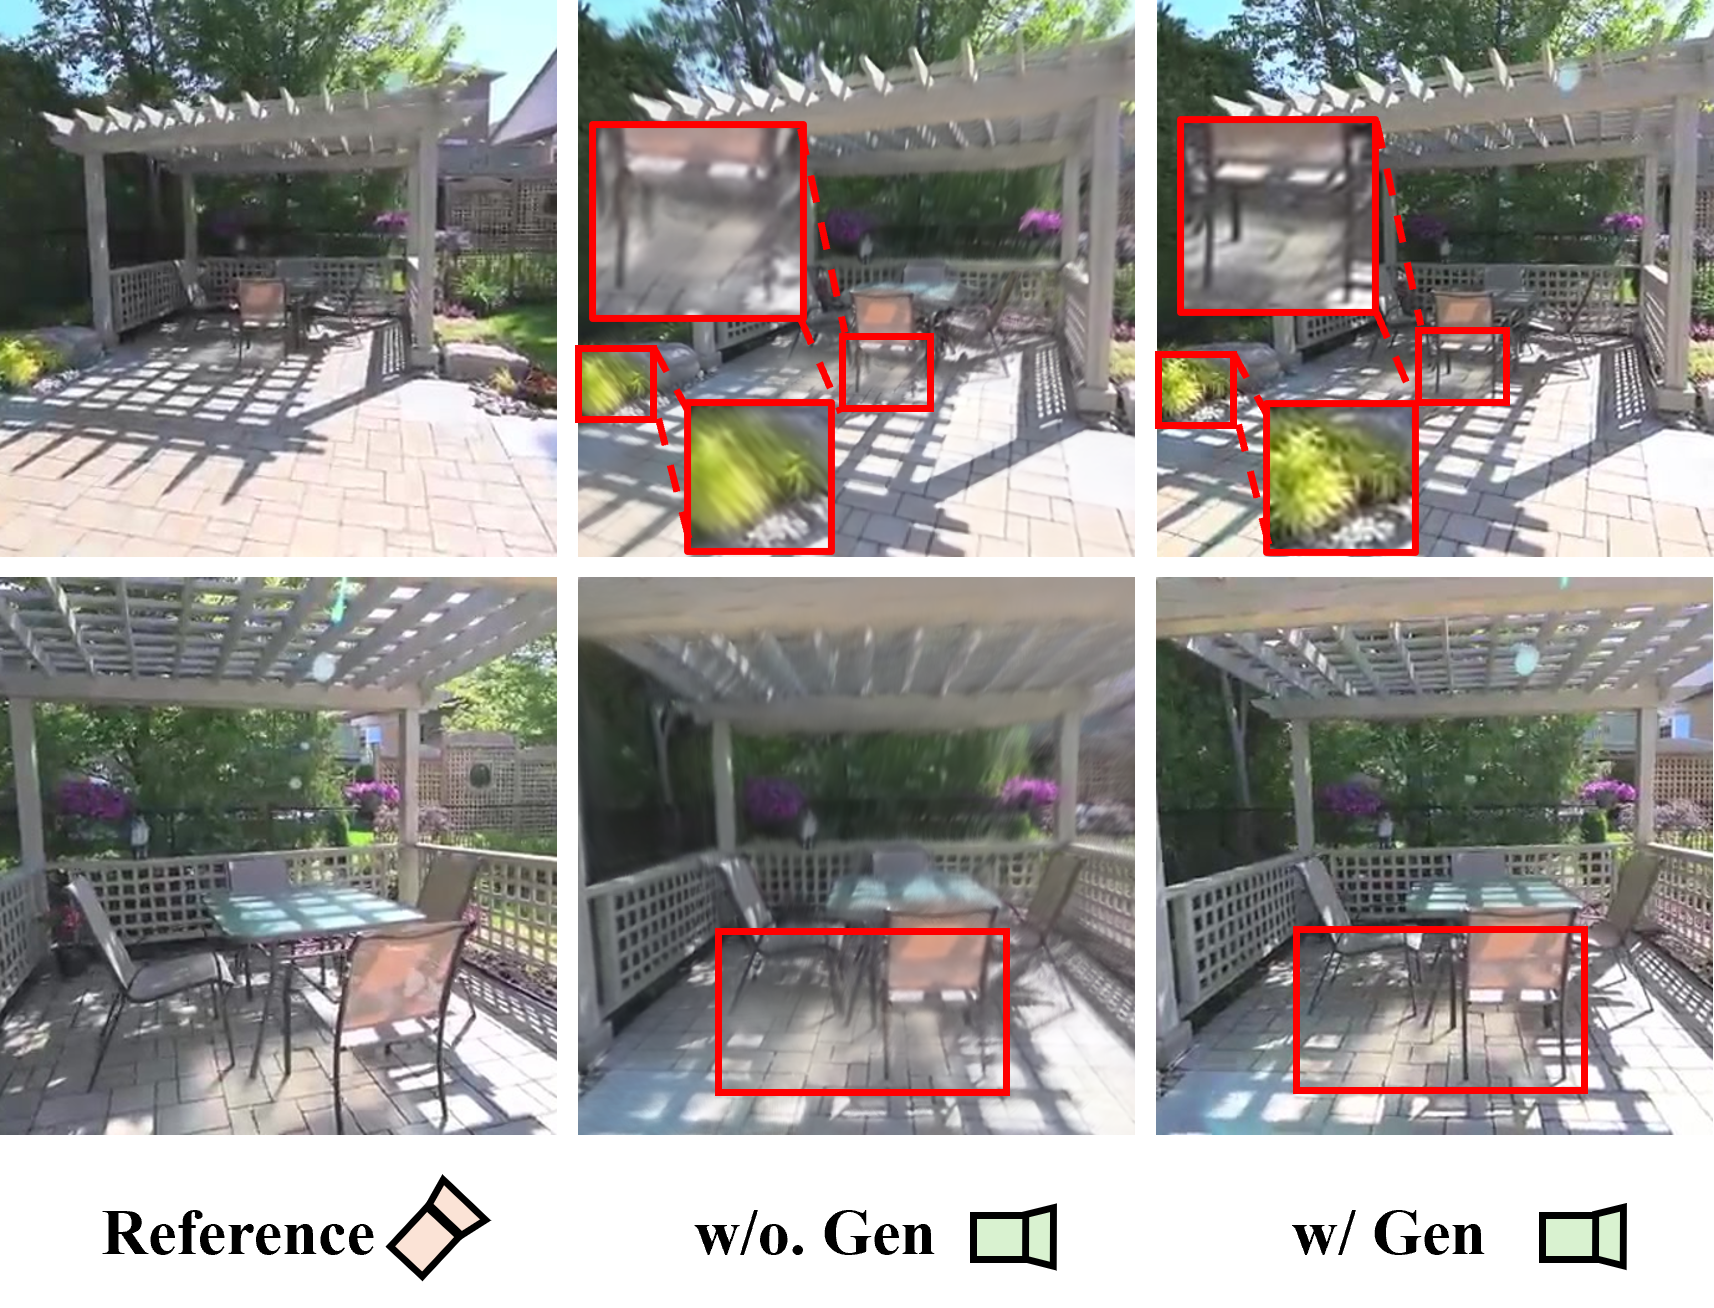
\includegraphics[width=0.95\columnwidth]{pics/difix.png}
  \caption{\textbf{Generative prior fusion.} Given sparse input views (left), our feed-forward 3DGS first produces a rendered view (middle). A frozen diffusion-based enhancer then refines this rendering into an enhanced image (right) with sharper textures and richer details, which is converted into Gaussian-level prior cues for subsequent residual updates.}
  \label{fig:difix}
\end{figure}


For each $m\in\mathcal{S}^{(t)}$, we enhance the current rendering using a diffusion-based enhancer $\mathcal{E}_\phi$ and pretrained model Difix \cite{wu2025difix3d+}: $\tilde{R}_m^{(t)}=\mathcal{E}_\phi\!\big(R_m^{(t)}\big).$
We compute a prior difference in feature space: $P_m^{(t)}=\psi\!\big(\tilde{R}_m^{(t)}\big)-\psi\!\big(R_m^{(t)}\big).$ Then pooling to Gaussians mirrors the evidence pooling to get $\mathbf{p}_i^{(t)}$. These cues regularize forward updates of $U_\theta$ under domain shift and provide high-frequency hints in under-constrained regions. The generative prior cues are similar to observed cues.
\begin{equation}
\mathbf{p}_i^{(t)} \;=\;
\frac{\sum_{m\in\mathcal{S}^{(t)}}\sum_{u} w_i(u)\,P_m^{(t)}(u)}
     {\sum_{m\in\mathcal{S}^{(t)}}\sum_{u} w_i(u)+\varepsilon}.
\end{equation}

We fuse observation-driven evidence and prior cues by concatenation at the gaussian level.
\begin{equation}
\Delta \mathcal{G}_i^{(t)} \;=\; U_\theta\big(\,[g_i^{(t)} \,\|\, \{o_i\}^{(t)} \,\|\, \{p_i\}^{(t)}]\,\big),
\end{equation}
\begin{equation}
    \mathcal{G}^{(t+1)}=\mathcal{G}^{(t)}+\Delta\mathcal{G}^{(t)}.,\quad t=0,\dots,T-1,
\end{equation}
where $g_i^{(t)}$ denotes the Gaussian-state including current per-gaussian parameters and corresponding features, $\{o_i\}^{(t)}$ the observation cues are distilled from rendered–image feature differences, and $\{p_i\}^{(t)}$ the prior cues distilled from diffusion-enhanced renderings. We do not implement gradient backpropagation through single-step diffusion model $\mathcal{E}_\phi$, the prior serves only as a forward cue. 

Our framework enables feed-forward efficiency, scene-adaptive refinement, and use of generative priors without ever-increasing view synthesis or test-time gradient updates, scales roughly linearly with $T$ and the per-iteration view budget, and improves robustness under domain shift via the refinement by observed cue and generative prior. 


\subsection{Loss Functions}
\label{sec:loss}

We train in two stages, applying geometric
distillation $\mathcal{L}_{\mathrm{dist}}$ as \cite{jiang2025anysplat} and photometric loss in novel view during Stage~I to bootstrap a stable initialization.
%Let $R_m^{(t)} = \mathcal{R}(\mathcal{G}^{(t)};\Pi_m)$ denote the rendering at iteration $t$.

In stage 1 initialization ($t{=}0$), we supervise the first forward prediction with a pixel reconstruction loss $\mathcal{L}_{\mathrm{rec}}$%, we additionally distill basic geometric cues use $\mathcal{L}_{\mathrm{dist}}$ in \cite{jiang2025anysplat}.
\begin{equation}
\mathcal{L}_{\mathrm{rec}} =
\lambda_{\mathrm{rgb}}\|I_m - R_m\|_2.
\end{equation}
\begin{equation}
    \mathcal{L}_{\mathrm{stage1}}
=\sum_{m\in\mathcal{M}}\big(
\mathcal{L}_{\mathrm{rec}}+\mathcal{L}_{\mathrm{dist}}
\big).
\end{equation}

In stage 2 refinement ($t{>}0$), we unroll $T$ forward-only refinement steps and supervise each rendering using
the multi-steps render loss $ \mathcal{L}_{\mathrm{stage2}}$. More details are stated in Appendix.
\begin{equation}
    \mathcal{L}_{\mathrm{stage2}}
=\sum_{t=1}^{T}\omega_t\sum_{m\in\mathcal{M}}
\|I_m - R_m^{(t)}\|_2.
\end{equation}
